\subsection{Pianificazione dei test}
La consistenza dei test in esecuzioni ripetute è una condizione imperativa, dunque è necessario che essi siano \gl{ripetibili}: un dato test eseguito in un ambiente specifico deve produrre, se fornito un determinato input, sempre gli stessi output. Al fine di garantire ciò, il team 7DOS ha scelto di basarsi sullo standard \gl{ISO/IEC/IEEE 29119}\footnote{ISO/IEC/IEEE 29119 parte 3 sezione 7, IEEE 2013.} per quanto riguarda la pianificazione e documentazione dei test dinamici. Tale standard prevede di definire, per ciascun test o suite di test, una \emph{specifica di test} composta di:
\begin{itemize}
	\item {\textbf{Specifica di progettazione:} definisce le funzionalità del prodotto da testare e le condizioni di test, ovvero l'ambiente di esecuzione e le pre-condizioni (particolari eventi o stati pregressi) necessarie al suo svolgimento;}
	\item {\textbf{Specifica di caso:} definisce l'insieme degli input che si desidera testare, e l'insieme dei risultati attesi per ogni (gruppo di) input per una o più funzionalità testate;}
	\item {\textbf{Specifica di procedura:} definisce l'ordine di esecuzione dei test (nel caso di una suite di test), la modalità di svolgimento, ovvero le azioni da compiere e gli input da inserire in modo ordinato, eventuali azioni necessarie per il raggiungimento delle pre-condizioni e la modalità di analisi dei risultati ottenuti.}
\end{itemize}

Per quanto concerne la \emph{specifica di progettazione}, il team ha scelto di associarvi uno o più requisiti funzionali a seconda della specificità del test, descritti nell'\emph{Analisi dei Requisiti v3.0.0}. Questo permette di descrivere più precisamente le funzionalità oggetto di test e di tracciare al meglio il soddisfacimento dei requisiti. \\

\subsubsection{Test di accettazione}
\normalsize
\renewcommand{\arraystretch}{1}
\begin{longtable}{|C{2.5cm}|C{2.5cm}|L{6.5cm}|C{1.5cm}|}
	\hline
	\rowcolor{title_row}
	\textbf{\color{title_text}{Test}} & \textbf{\color{title_text}{Requisito}} & \textbf{\color{title_text}{Descrizione}} & \textbf{\color{title_text}{Stato}} \\
	\hline
	\endhead
	{TA-1} & {R0F1} & 
	Verifica che il sistema permetta di leggere la definizione di una rete Bayesiana importando un file in formato JSON.
	\textbf{Procedura}:
	\begin{itemize}		
		\item L'utente crea un nuovo 7DOS panel;
		\item L'utente si posiziona sulla scheda di \emph{"Edit"};
		\item L'utente si posiziona sul \emph{"JSON import"} panel;
		\item L'utente preme il pulsante per importare un file JSON;
		\item L'utente seleziona il file da importare;
		\item Conferma la selezione del file;
		\item Il sistema importa la definizione della rete mostrandone il contenuto.
	\end{itemize}
	  & {NI}\\
	\hline
	{TA-1.1} & {R1F1.1} & Verifica che il sistema permetta di verificare se un file JSON sia valido.
	\textbf{Procedura}:
	\begin{itemize}		
		\item L'utente crea un nuovo 7DOS panel;
		\item L'utente si posiziona sulla scheda di \emph{"Edit"};
		\item L'utente si posiziona sul \emph{"JSON import"} panel;
		\item L'utente preme il pulsante per importare un file JSON;
		\item L'utente seleziona il file non valido da importare;
		\item Conferma la selezione del file;
		\item Il sistema mostra un messaggio di errore e l'importazione del file non è andata a buon fine.
	\end{itemize}
	 & {NI}\\
	\hline
	{TA-2} & {R0F2} & 
	Verifica che il sistema permetta la gestione della connessione tra i nodi della rete ed il flusso di dati.
	\textbf{Procedura}:
	\begin{itemize}		
		\item L'utente si posiziona sulla scheda di \emph{"Edit"};
		\item L'utente si posiziona sul \emph{"Network"} panel;
		\item L'utente seleziona il flusso di dati da monitorare.
	\end{itemize}
	 & {NI}\\
	\hline
	{TA-2.1} & {R0F2.1} & 
	Verifica che il sistema permetta di connettere un nodo della rete al flusso di dati.
	\textbf{Procedura}:
	\begin{itemize}		
		\item L'utente si posiziona sulla scheda di \emph{"Edit"};
		\item L'utente si posiziona sul \emph{"Network"} panel;
		\item L'utente seleziona il nodo da monitorare rispetto al flusso di dati.
	\end{itemize}
	 & {NI}\\
	\hline
	{TA-2.2} & {R0F2.2} & 
	Verifica che il sistema permetta di disconnettere un nodo della rete al flusso di dati.
	\textbf{Procedura}:
	\begin{itemize}		
		\item L'utente si posiziona sulla scheda di \emph{"Edit"};
		\item L'utente si posiziona sul \emph{"Network"} panel;
		\item L'utente deseleziona il nodo da monitorare rispetto al flusso di dati.
	\end{itemize}
	 & {NI}\\
	\hline
	{TA-2.3} & {R1F2.3} & 
	Verifica che il sistema permetta di modificare un nodo della rete connesso al flusso di dati.
	\textbf{Procedura}:
	\begin{itemize}		
		\item L'utente si posiziona sulla scheda di \emph{"Edit"};
		\item L'utente si posiziona sul \emph{"Network"} panel;
		\item L'utente modifica il nodo da monitorare rispetto al flusso di dati.
	\end{itemize}
	 & {NI}\\
	\hline
	{TA-3} & {R0F3} & 
	Verifica che il sistema permetta di applicare il
	ricalcolo delle probabilità della rete
	secondo regole temporali stabilite dall'utente.
	\textbf{Procedura}:
	\begin{itemize}		
		\item L'utente si posiziona sulla scheda di \emph{"Edit"};
		\item L'utente si posiziona sul \emph{"Network"} panel;
		\item Il sistema effettua il ricalcolo delle probabilità della rete aggiornandone lo stato dei nodi.
	\end{itemize}	
	 & {NI}\\
	\hline
	{TA-3.1} & {R1F3.1} & 
	Verifica che il sistema permetta all'utente di modificare le regole temporali per effettuare il ricalcolo delle probabilità della rete.
	\textbf{Procedura}:
	\begin{itemize}		
		\item L'utente si posiziona sulla scheda di \emph{"Edit"};
		\item L'utente si posiziona sul \emph{"Network"} panel;
		\item L'utente modifica le regole temporali per il ricalcolo delle probabilità della rete.
	\end{itemize}
	 & {NI}\\
	\hline
	{TA-4} & {R0F4} & 
	Verifica che il sistema permetta fornire nuovi dati a Grafana derivati dai nodi
	della rete non direttamente collegati al flusso di
	dati.
	\textbf{Procedura}:
	\begin{itemize}		
		\item ;
		\item ;
		\item .
	\end{itemize}
	 & {NI}\\
	\hline
	{TA-4.1} & {R1F4.1} & 
	Verifica che il sistema permetta l'aggiornamento dei dati secondo una frequenza stabilita dall'utente.
	\textbf{Procedura}:
	\begin{itemize}		
		\item ;
		\item ;
		\item .
	\end{itemize}
	& {NI}\\
	\hline
	{TA-5} & {R0F5} & 
	Verifica che il sistema permetta di leggere i dati provenienti dal flusso ed elaborarli, visualizzandone il risultato attraverso un grafico.
	\textbf{Procedura}:
	\begin{itemize}		
		\item Il sistema legge i dati proveniente dal flusso;
		\item Il sistema effettua il ricalcolo delle probabilità della rete aggiornando lo stato dei nodi;
		\item Il sistema elabora i risultati e li mostra attraverso un grafico.
	\end{itemize}
	 & {NI}\\
	\hline
	{TA-5.1} & {R1F5.1} & 
	Verifica che il sistema aggiorni i dati presenti nel grafico in base alla frequenza stabilita dall'utente.
	\textbf{Procedura}:
	\begin{itemize}		
		\item Il sistema legge i nuovi dati proveniente dal flusso, in base alla frequenza stabilita;
		\item Il sistema effettua il ricalcolo delle probabilità della rete aggiornando lo stato dei nodi, in base alla frequenza stabilita;
		\item Il sistema elabora i risultati e li mostra attraverso un grafico.
	\end{itemize}
	 & {NI}\\
	\hline
	{TA-5.2} & {R1F5.2} & 
	Verifica che il sistema permetta all'utente di creare un nuovo panel.
	\textbf{Procedura}:
	\begin{itemize}		
		\item L'utente si posiziona all'interno di una dashboard;
		\item L'utente clicca sulla voce \emph{add panel};
		\item L'utente sceglie la tipologia di panel da creare;
		\item Il sistema crea il nuovo panel e lo mostra all'interno della dashboard.
	\end{itemize}
	 & {NI}\\
	\hline
	{TA-5.3} & {R1F5.3} & 
	Verifica che il sistema permetta all'utente di spostare un panel all'interno della dashboard.
	\textbf{Procedura}:
	\begin{itemize}		
		\item L'utente si posiziona all'interno di una dashboard;
		\item L'utente trascina il panel che vuole spostare nella posizione desiderata;
		\item Il sistema sposta panel nella nuova posizione scelta dall'utente.
	\end{itemize}
	 & {NI}\\
	\hline
	{TA-5.4} & {R1F5.4} & 
	Verifica che il sistema permetta all'utente di cancellare un panel all'interno della dashboard.
	\textbf{Procedura}:
	\begin{itemize}		
		\item L'utente si posiziona all'interno di una dashboard;
		\item L'utente clicca sull'intestazione del panel;
		\item L'utente seleziona la voce \emph{"Remove"};
		\item Conferma l'eliminazione del panel;
		\item Il sistema cancella panel scelto dall'utente.
	\end{itemize}
	 & {NI}\\
	\hline
	{TA-5} & {R1F5.5} & 
	Verifica che il sistema permetta all'utente di minimizzare un panel.
	\textbf{Procedura}:
	\begin{itemize}		
		\item L'utente si posiziona all'interno di una dashboard;
		\item L'utente si posiziona sull'angolo in basso a destra del panel;
		\item L'utente modifica minimizza il panel;
		\item Il sistema modifica la dimensione del panel come scelto dall'utente.
	\end{itemize}
	 & {NI}\\
	\hline
	{TA-5.6} & {R1F5.6} & 
	Verifica che il sistema permetta all'utente configurare un panel dopo la sua creazione.
	\textbf{Procedura}:
	\begin{itemize}		
		\item L'utente si posiziona all'interno di una dashboard;
		\item L'utente configura le opzioni del panel come desidera;
		\item Il sistema configura le opzioni del panel come stabilito dall'utente.
	\end{itemize}
	 & {NI}\\
	\hline
	{TA-5.7} & {R1F5.7} & 
	Verifica che il sistema permetta all'utente di modificare un panel all'interno della dashboard.
	\textbf{Procedura}:
	\begin{itemize}		
		\item L'utente si posiziona all'interno di una dashboard;
		\item L'utente modifica le opzioni del panel come desidera;
		\item Il sistema modifica le opzioni del panel come stabilito dall'utente.
	\end{itemize}
	 & {NI}\\
	\hline
	{TA-6} & {R1F6} & 
	Verifica che il sistema permetta all'utente di definire alert in base a livelli di soglia raggiunti dai nodi non collegati al flusso dei dati.
	\textbf{Procedura}:
	\begin{itemize}		
		\item L'utente si posiziona all'interno di un panel di tipo \emph{graph};
		\item L'utente si posiziona sulla schermata di \emph{edit};
		\item L'utente si posiziona sulla scheda \emph{"Alert"};
		\item L'utente clicca sul pulsante \emph{"Create alert"};
		\item Il sistema crea un nuovo alert.
	\end{itemize}
	 & {NI}\\
	\hline
	{TA-6.1} & {R1F6.1} & 
	Verifica che il sistema permetta all'utente di configurare i parametri di un alert.
	\textbf{Procedura}:
	\begin{itemize}		
		\item L'utente si posiziona sulla scheda \emph{"Alert"};
		\item L'utente seleziona l'alert da configurare;
		\item L'utente configura i parametri come desidera;
		\item Il sistema configura i parametri dell'alert.
	\end{itemize}
	 & {NI}\\
	\hline
	{TA-6.2} & {R1F6.2} & 
	Verifica che il sistema permetta all'utente di impostare il modo in cui viene notificata l'attivazione di un alert.
	\textbf{Procedura}:
	\begin{itemize}		
		\item L'utente si posiziona sulla scheda \emph{"Alert"};
		\item L'utente seleziona l'alert da configurare;
		\item L'utente imposta come deve venire notificata l'attivazione dell'alert;
		\item Il sistema imposta il sistema di notifica dell'alert.
	\end{itemize}
	 & {NI}\\
	\hline
	{TA-7} & {R1F7} & 
	Verifica che il sistema permetta di disegnare una rete Bayesiana con un editor grafico specializzato.
	\textbf{Procedura}:
	\begin{itemize}		
		\item ;
		\item ;
		\item .
	\end{itemize}
	 & {NI}\\
	\hline
	{TA-7.1} & {R1F7.1} & 
	Verifica che il sistema permetta di creare un nuovo nodo della rete.
	\textbf{Procedura}:
	\begin{itemize}		
		\item ;
		\item ;
		\item .
	\end{itemize}
	 & {NI}\\
	\hline
	{TA-7.2} & {R1F7.2} & 
	Verifica che il sistema permetta di modificare i parametri di un nodo della rete.
	\textbf{Procedura}:
	\begin{itemize}		
		\item ;
		\item ;
		\item .
	\end{itemize}
	 & {NI}\\
	\hline
	{TA-7.4} & {R1F7.4} & 
	Verifica che il sistema permetta di creare un collegamento tra due nodi della rete.
	\textbf{Procedura}:
	\begin{itemize}		
		\item ;
		\item ;
		\item .
	\end{itemize}
	 & {NI}\\
	\hline
	{TA-7.5} & {R1F7.5} & 
	Verifica che il sistema permetta di eliminare un collegamento tra due nodi della rete.
	\textbf{Procedura}:
	\begin{itemize}		
		\item ;
		\item ;
		\item .
	\end{itemize}
	 & {NI}\\
	\hline
	{TA-7.6} & {R1F7.6} & 
	Verifica che il sistema permetta di salvare la rete realizzata su un file JSON.
	\textbf{Procedura}:
	\begin{itemize}		
		\item ;
		\item ;
		\item .
	\end{itemize}
	 & {NI}\\
	\hline
	{TA-7.7} & {R1F7.7} & 
	Verifica che il sistema rilevi e sia in grado di gestire eventuali errori derivati dalla modifica di un nodo.
	\textbf{Procedura}:
	\begin{itemize}		
		\item ;
		\item ;
		\item .
	\end{itemize}
	 & {NI}\\
	\hline
	{TA-8} & {R2F8} & 
	Verifica che il sistema permetta di applicare più reti Bayesiane a diversi oggetti di monitoraggio.
	\textbf{Procedura}:
	\begin{itemize}		
		\item ;
		\item ;
		\item .
	\end{itemize}
	 & {NI}\\
	\hline
	{TA-9} & {R2F9} & 
	Verifica che il sistema permetta di creare una rete Bayesiana a partire dai dati raccolti
	sul campo.
	\textbf{Procedura}:
	\begin{itemize}		
		\item ;
		\item ;
		\item .
	\end{itemize}
	 & {NI}\\
	\hline
	{TA-10} & {R2F10} & 
	Verifica che il sistema permetta di condividere grafici presenti in una dashboard o in un singolo panel.
	\textbf{Procedura}:
	\begin{itemize}		
		\item L'utente si posiziona all'interno di una dashboard;
		\item L'utente seleziona l'opzione \emph{"Share"} relativa alla dashboard o ad un panel;
		\item Il sistema condivide il grafico secondo l'opzione scelta dall'utente.
	\end{itemize}
	 & {NI}\\
	\hline
	{TA-10.1} & {R2F10.1} & 
	Verifica che il sistema permetta di visualizzare il link diretto ad una dashboard o ad un
	panel.
	\textbf{Procedura}:
	\begin{itemize}		
		\item L'utente si posiziona all'interno di una dashboard;
		\item L'utente seleziona l'opzione \emph{"Share"} relativa alla dashboard o ad un panel;
		\item L'utente si posiziona sulla scheda \emph{"Link"};
		\item L'utente configura le opzioni per generare il link per la condivisione;
		\item Il sistema mostra il link generato con cui l'utente può effettuare la condivisione.
	\end{itemize}
	 & {NI}\\
	\hline
	{TA-10.2} & {R2F10.2} & 
	Verifica che il sistema permetta di visualizzare il codice per l'inclusione di un panel in una pagina web.
	\textbf{Procedura}:
	\begin{itemize}		
		\item L'utente si posiziona all'interno di una dashboard;
		\item L'utente seleziona l'opzione \emph{"Share"} relativa ad un panel;
		\item L'utente si posiziona sulla scheda \emph{"Embed"};
		\item L'utente configura le opzioni per generare il frame per la condivisione;
		\item Il sistema mostra il frame generato con cui l'utente può effettuare la condivisione.
	\end{itemize}
	 & {NI}\\
	\hline
	{TA-10.4} & {R2F10.4} & 
	Verifica che il sistema permetta di condividere lo snapshot di una dashboard o di un
	panel.

	\textbf{Procedura}:
	\begin{itemize}		
		\item L'utente si posiziona all'interno di una dashboard;
		\item L'utente seleziona l'opzione \emph{"Share"} relativa a una dashboard ad un panel;
		\item L'utente si posiziona sulla scheda \emph{"Snapshot"};
		\item L'utente configura le opzioni per la condivisione dello snapshot;
		\item Il sistema effettua la condivisione dello snapshot.
	\end{itemize}
	 & {NI}\\
	\hline
	{TA-10.5} & {R2F10.5} & 
	Verifica che il sistema permetta di visualizzare il codice JSON contenente la definizione
	di una dashboard.
	\textbf{Procedura}:
	\begin{itemize}		
		\item L'utente si posiziona all'interno di una dashboard;
		\item L'utente seleziona l'opzione \emph{"Share dashboard"};
		\item L'utente si posiziona sulla scheda \emph{"Export"};
		\item L'utente clicca sul pulsante per visualizzare il JSON;
		\item Il sistema mostra il codice JSON con la definizione della dashboard.
	\end{itemize}
	 & {NI}\\
	\hline
	{TA-10.6} & {R2F10.6} & 
	Verifica che il sistema permetta di salvare il file JSON contenente la definizione di una
	dashboard.
	\textbf{Procedura}:
	\begin{itemize}		
		\item L'utente si posiziona all'interno di una dashboard;
		\item L'utente seleziona l'opzione \emph{"Share dashboard"};
		\item L'utente si posiziona sulla scheda \emph{"Export"};
		\item L'utente clicca sul pulsante per salvare il JSON;
		\item Il sistema effettua il salvataggio del codice JSON con la definizione della dashboard.
	\end{itemize}
	 & {NI}\\
	\hline
	\caption{Riassunto test di accettazione}
	\label{tabella:riassunto ta}
\end{longtable}
\begin{figure} [H]
	\centering
	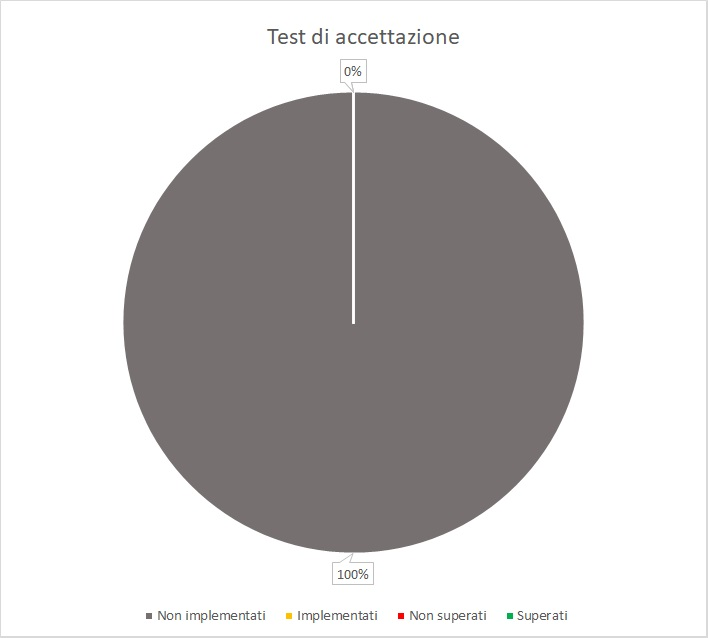
\includegraphics[scale=1]{Img/TA}
	\caption{Resoconto test di accettazione}\label{}
\end{figure}
\normalsize
\renewcommand{\arraystretch}{1}
\newpage

\definecolor{darkgreen}{rgb}{0.0, 0.6, 0.0}
\subsubsection{Test di sistema}
\begin{longtable}{|C{2.5cm}|C{2.5cm}|C{6.5cm}|C{1.5cm}|}
			\hline
			\rowcolor{title_row}
			\textbf{\color{title_text}{Test}} & \textbf{\color{title_text}{Requisito}} & \textbf{\color{title_text}{Descrizione}} & \textbf{\color{title_text}{Stato}} \\
			\hline
			\endhead
			{TS-0F1} & {R0F1} & Verifica che sia possibile e leggere la
			definizione della rete Bayesiana da un
			file in formato JSON.  & \textcolor{darkgreen}{\textbf{S}}\\
			\hline
			{TS-0F1.1} & {R1F1.1} & Verifica che sia possibile validare un
			file JSON. & {NI}\\
			\hline
			{TS-2} & {R0F2} & Verifica che sia possibile gestire la
			connessione tra i nodi della rete ai
			rispettivi flussi di dati. & {NI}\\
			\hline
			{TS-2.1} & {R0F2.1} & Verifica che sia possibile connettere un
			nodo della rete ad un flusso di dati. & {NI}\\
			\hline
			{TS-2.2} & {R0F2.2} & Verifica che sia possibile disconnettere un
			nodo della rete da un flusso di dati. & {NI}\\
			\hline
			{TS-2.3} & {R1F2.3} & Verifica che sia essere possibile modificare il
			flusso di dati connesso ad un nodo. & \textcolor{darkgreen}{\textbf{S}}\\
			\hline
			{TS-3} & {R0F3} & Verifica che sia possibile applicare il
			ricalcolo delle probabilità della rete
			secondo regole temporali prestabilite. & {NI}\\
			\hline
			{TS-3.1} & {R1F3.1} & Verifica che sia possibile modificare le
			suddette regole temporali. & {NI}\\
			\hline
			{TS-4} & {R0F4} & Verifica che sia possibile fornire nuovi dati
			al sistema di Grafana derivati dai nodi
			della rete non collegati al flusso di
			monitoraggio. & {NI}\\
			\hline
			{TS-4.1} & {R1F4.1} & Verifica che sia possibile aggiornare i dati
			in base alla frequenza stabilita. & \textcolor{darkgreen}{\textbf{S}}\\
			\hline
			{TS-5} & {R0F5} & Verifica che i dati siano disponibili al sistema di
			creazione di grafici e dashboard per la
			loro visualizzazione. & {NI}\\
			\hline
			{TS-5.1} & {R1F5.1} & Verifica che sia possibile aggiornare la
			dashboard in base alla frequenza
			stabilita. & \textcolor{darkgreen}{\textbf{S}}\\
			\hline
			{TS-5.2} & {R1F5.2} & Verifica che sia possibile creare un panel. & \textcolor{darkgreen}{\textbf{S}}\\
			\hline
			{TS-5.3} & {R1F5.3} & Verifica che sia possibile spostare un
			panel. & \textcolor{darkgreen}{\textbf{S}}\\
			\hline
			{TS-5.4} & {R1F5.4} & Verifica che sia possibile cancellare un
			panel. & \textcolor{darkgreen}{\textbf{S}}\\
			\hline
			{TS-5.5} & {R1F5.5} & Verifica che sia possibile minimizzare un
			panel. & \textcolor{darkgreen}{\textbf{S}}\\
			\hline
			{TS-5.6} & {R1F5.6} & Verifica che sia possibile configurare un
			panel. & \textcolor{darkgreen}{\textbf{S}}\\
			\hline
			{TS-5.6.1} & {R0F5.6.1} & Verifica che sia possibile selezionare un
			flusso dati. & {NI}\\
			\hline
			{TS-5.6.2} & {R1F5.6.2} & Verifica che sia selezionare un
			nodo della rete. & {NI}\\
			\hline
			{TS-5.6.3} & {R1F5.6.3} & Verifica che sia possibile selezionare un
			intervallo di tempo.  & \textcolor{darkgreen}{\textbf{S}}\\
			\hline
			{TS-5.7} & {R1F5.7} & Verifica che sia possibile modificare un
			panel.  & \textcolor{darkgreen}{\textbf{S}}\\
			\hline
			{TS-5.7.1} & {R1F5.7.1} & Verifica che sia possibile usare le
			modifiche standard di Grafana su un
			panel. & \textcolor{darkgreen}{\textbf{S}}\\
			\hline
			{TS-6} & {R1F6} & Verifica che sia  possibile definire alert in
			base a livelli di soglia raggiunti dai
			nodi non collegati al flusso dei dati.  & \textcolor{darkgreen}{\textbf{S}}\\
			\hline
			{TS-6.1} & {R1F6.1} & Verifica che sia possibile configurare i
			parametri di un alert.  & \textcolor{darkgreen}{\textbf{S}}\\
			\hline
			{TS-6.1.1} & {R1F6.1.1} & Verifica che sia possibile inserire il nome
			di un alert.  & \textcolor{darkgreen}{\textbf{S}}\\
			\hline
			{TS-6.1.2} & {R1F6.1.2} & Verifica che sia  possibile inserire
			l'intervallo di verifica di un alert.  & \textcolor{darkgreen}{\textbf{S}}\\
			\hline
			{TS-6.1.3} & {R1F6.1.3} & Verifica che sia possibile inserire la
			condizione di attivazione di un alert.  & \textcolor{darkgreen}{\textbf{S}}\\
			\hline
			{TS-6.2} & {R1F6.2} & Verifica che sia possibile impostare il
			modo in cui viene notificata
			l'attivazione di un alert.  & \textcolor{darkgreen}{\textbf{S}}\\
			\hline
			{TS-7} & {R1F7} & Verifica che sia possibile disegnare la rete
			Bayesiana con un editor
			grafico specializzato.  & {NI}\\
			\hline
			{TS-7.1} & {R1F7.1} & Verifica che sia possibile creare un nodo
			della rete.  & {NI}\\
			\hline
			{TS-7.11} & {R1F7.1.1} & Verifica che sia  possibile inizializzare la lista di predecessori
			del nodo.  & {NI}\\
			\hline
			{TS-7.1.2} & {R1F7.1.2} & Verifica che sia possibile inizializzare la lista di successori del
			nodo.  & {NI}\\
			\hline
			{TS-7.1.3} & {R1F7.1.3} & Verifica che sia possibile inizializzare il nome del nodo.  & {NI}\\
			\hline
			{TS-7.1.4} & {R1F7.1.4} & Verifica che sia possibile inizializzare la CPT associata al
			nodo.  & {NI}\\
			\hline
			{TS-7.1.4.1} & {R1F7.1.4.1} & Verifica che sia possibile inizializzare la lista degli stati
			associata alla CPT del nodo.  & {NI}\\
			\hline
			{TS-7.1.4.2} & {R1F7.1.4.2} & Verifica che sia possibile inizializzare la lista delle
			combinazioni degli stati dei nodi
			predecessori associata alla CPT del
			nodo.  & {NI}\\
			\hline
			{TS-7.1.4.3} & {R1F7.1.4.3} & Verifica che sia possibile inizializzare le celle della CPT.  & {NI}\\
			\hline
			{TS-7.2} & {R1F7.2} & Verifica che sia possibile modificare i
			parametri di un nodo della rete.  & {NI}\\
			\hline
			{TS-7.2.1} & {R1F7.2.1} & Verifica che sia  possibile modificare il
			nome di un nodo della rete.  & {NI}\\
			\hline
			{TS-7.2.2} & {R1F7.2.2} & Verifica che sia possibile modificare la
			CPT associata ad un nodo della rete.  & {NI}\\
			\hline
			{TS-7.2.2.1} & {R1F7.2.2.1} & Verifica che sia possibile aggiungere uno
			stato alla CPT associata ad un nodo
			della rete.
  & {NI}\\
			\hline
			{TS-7.2.2.2} & {R1F7.2.2.2} & Verifica che sia possibile eliminare uno
			stato dalla CPT associata ad un nodo
			della rete.  & {NI}\\
			\hline
			{TS-7.2.2.3} & {R1F7.2.2.3} & Verifica che sia possibile modificare i
			parametri associati ad uno stato della
			CPT associata ad un nodo della rete.  & {NI}\\
			\hline
			{TS-7.2.2.4} & {R1F7.2.2.4} & Verifica che sia possibile modificare una
			cella della CPT.  & {NI}\\
			\hline
			{TS-7.3} & {R1F7.3} & Verifica che sia possibile eliminare un
			nodo dalla rete.  & {NI}\\
			\hline
			{TS-7.4} & {R1F7.4} & Verifica che sia possibile creare un
			collegamento tra due nodi della rete.  & {NI}\\
			\hline
			{TS-7.4.1} & {R1F7.4.1} & Verifica che sia possibile indicare il nodo
			di partenza del collegamento.  & {NI}\\
			\hline
			{TS-7.4.2} & {R1F7.4.2} & Verifica che sia possibile indicare il nodo
			di arrivo del collegamento.  & {NI}\\
			\hline
			{TS-7.5} & {R1F7.5} & Verifica che sia possibile eliminare un
			collegamento dalla rete.  & {NI}\\
			\hline
			{TS-7.6} & {R1F7.6} & Verifica che sia possibile salvare la rete su
			file JSON.  & {NI}\\
			\hline
			{TS-7.6.1} & {R1F7.6.1} & Verifica che sia possibile indicare il nome
			del file JSON su cui si vuole salvare la
			struttura della rete.  & {NI}\\
			\hline
			{TS-7.6.2} & {R1F7.6.2} & Verifica che sia possibile indicare il
			percorso del file system in cui si vuole
			salvare il file JSON contenente la
			struttura della rete.  & {NI}\\
			\hline
			{TS-7.7} & {R1F7.7} & Verifica che sia possibile gestire errori
			relativi alla modifica di un nodo.  & {NI}\\
			\hline
			{TS-7.7.1} & {R1F7.7.1} & Verifica che sia  possibile gestire
			l'inserimento di valori non validi per il
			nome di un nodo.  & {NI}\\
			\hline
			{TS-7.7.2} & {R1F7.7.2} & Verifica che sia possibile gestire
			l'inserimento di valori non validi per il
			nome di uno stato associato alla CPT
			di un nodo della rete  & {NI}\\
			\hline
			{TS-7.7.3} & {R1F7.7.3} & Verifica che sia possibile gestire
			l'inserimento di valori non validi per
			l'intervallo associato ad uno stato del
			nodo.
  & {NI}\\
			\hline
			{TS-7.7.4} & {R1F7.7.4} & Verifica che sia e possibile gestire
			l'inserimento di valori non validi per
			una cella della tabella.  & {NI}\\
			\hline
			{TS-8} & {R2F8} & Verifica che sia possibile applicare più reti
			Bayesiane in oggetti di monitoraggio
			diversi.  & {NI}\\
			\hline
			{TS-9} & {R2F9} & Verifica che sia  possibile creare una rete
			Bayesiana a partire dai dati raccolti
			sul campo anziché svilupparla con la
			collaborazione degli esperti del settore.  & {NI}\\
			\hline
			{TS-10} & {R2F10} & Verifica che sia possibile condividere un
			grafico.  & \textcolor{darkgreen}{\textbf{S}}\\
			\hline
			{TS-10.1} & {R2F10.1} & Verifica che sia possibile visualizzare il
			link diretto ad una dashboard o ad un
			panel.  & \textcolor{darkgreen}{\textbf{S}}\\
			\hline
			{TS-10.2} & {R2F10.2} & Verifica che sia  possibile visualizzare il
			codice per l’inclusione di un panel in
			una pagina web.  & \textcolor{darkgreen}{\textbf{S}}\\
			\hline
			{TS-10.3} & {R2F10.3} & Verifica che sia possibile selezionare le
			opzioni di visualizzazione per la
			condivisione dei grafici.
  & \textcolor{darkgreen}{\textbf{S}}\\
			\hline
			{TS-10.3.1} & {R2F10.3.1} & Verifica che sia  possibile selezionare la
			visualizzazione dell'intervallo di tempo
			corrente in un grafico.  & \textcolor{darkgreen}{\textbf{S}}\\
			\hline
			{TS-10.3.2} & {R2F10.3.2} & Verifica che sia  possibile deselezionare la
			visualizzazione dell'intervallo di tempo
			corrente in un grafico.
  & \textcolor{darkgreen}{\textbf{S}}\\
			\hline
			{TS-10.3.3} & {R2F10.3.3} & Verifica che sia possibile selezionare la
			visualizzazione di variabili di template
			in un grafico.  & \textcolor{darkgreen}{\textbf{S}}\\
			\hline
			{TS-10.3.4} & {R2F10.3.4} & Verifica che sia  possibile deselezionare la
			visualizzazione di variabili di template
			in un grafico.  & \textcolor{darkgreen}{\textbf{S}}\\
			\hline
			{TS-10.3.5} & {R2F10.3.5} & Verifica che sia possibile selezionare il
			tema di un grafico.  & \textcolor{darkgreen}{\textbf{S}}\\
			\hline
			{TS-10.4} & {R2F10.4} & Verifica che sia possibile condividere uno
			snapshot di una dashboard o di un
			panel.  & \textcolor{darkgreen}{\textbf{S}}\\
			\hline
			{TS-10.4.1} & {R2F10.4.1} & Verifica che sia possibile pubblicare uno
			snapshot sull'istanza locale dell'utente.   & \textcolor{darkgreen}{\textbf{S}}\\
			\hline
			{TS-10.4.2} & {R2F10.4.2} & Verifica che sia possibile pubblicare uno
			snapshot su Raintank.  & \textcolor{darkgreen}{\textbf{S}}\\
			\hline
			{TS-10.4.3} & {R2F10.4.3} & Verifica che sia possibile configurare le
			opzioni di visualizzazione di uno
			snapshot.
  & \textcolor{darkgreen}{\textbf{S}}\\
			\hline
			{TS-10.4.3.1} & {R2F10.4.3.1} & Verifica che sia possibile inserire il nome
			di uno snapshot.  & \textcolor{darkgreen}{\textbf{S}}\\
			\hline
			{TS-10.4.3.2} & {R2F10.4.3.2} & Verifica che sia possibile selezionare il
			tempo di permanenza di uno snapshot.  & \textcolor{darkgreen}{\textbf{S}}\\
			\hline
			{TS-10.4.3.3} & {R2F10.4.3.3} & Verifica che sia possibile inserire il tempo
			massimo per il caricamento dei dati in
			uno snapshot.
  & \textcolor{darkgreen}{\textbf{S}}\\
			\hline
			{TS-10.5} & {R2F10.5} & Verifica che sia possibile visualizzare il
			codice JSON contenente la definizione
			di una dashboard.  & \textcolor{darkgreen}{\textbf{S}}\\
			\hline
			{TS-10.6} & {R2F10.6} & Verifica che sia possibile salvare il file
			JSON contenente la definizione di una
			dashboard.  & \textcolor{darkgreen}{\textbf{S}}\\
			\hline
	\caption{Riassunto test di sistema}
	\label{tabella:riassunto TS}
\end{longtable}
\renewcommand{\arraystretch}{1}
\begin{figure} [H]
	\centering
	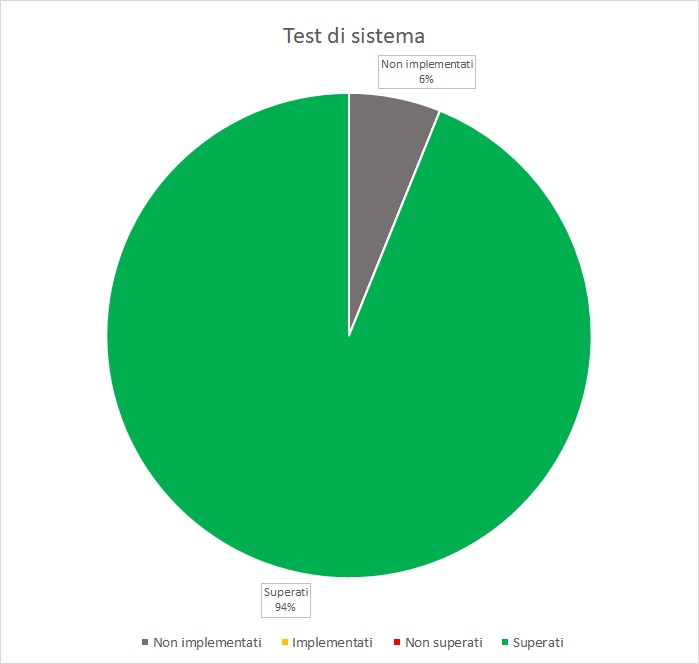
\includegraphics[scale=1]{Img/TS}
	\caption{Resoconto test di sistema}\label{}
\end{figure}
\newpage

\subsubsection{Test di integrazione}
\normalsize
\renewcommand{\arraystretch}{1}
\begin{longtable}{|C{2.5cm}|C{6.5cm}|C{1.5cm}|}
	\hline
	\rowcolor{title_row}
	\textbf{\color{title_text}{Test}} & \textbf{\color{title_text}{Descrizione}} & \textbf{\color{title_text}{Stato}} \\
	\hline
	\endhead
	{TI-1} & Verifica l'integrazione tra client e Grafana. & \textcolor{darkgreen}{\textbf{S}}\\
	\hline
	{TI-2} & Verifica l'integrazione tra Grafana ed \gl{InfluxDB}. & \textcolor{darkgreen}{\textbf{S}}\\
	\hline
	{TI-3} & Verifica l'integrazione tra Grafana e JsBayes. & \textcolor{darkgreen}{\textbf{S}}\\
	\hline
	{TI-4} & Verifica l'integrazione tra Grafana e Raintank. & \textcolor{darkgreen}{\textbf{S}}\\
	\hline
	\caption{Riassunto test di integrazione}
	\label{tabella:riassunto ta}
\end{longtable}
\renewcommand{\arraystretch}{1}
\begin{figure} [H]
	\centering
	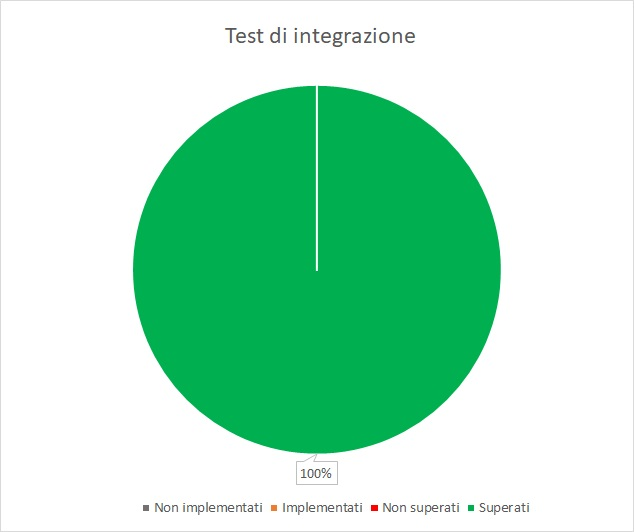
\includegraphics[scale=1]{Img/TI}
	\caption{Resoconto test di integrazione}\label{}
\end{figure}
\newpage

\subsubsection{Test di unità}
\begin{figure} [H]
	\centering
	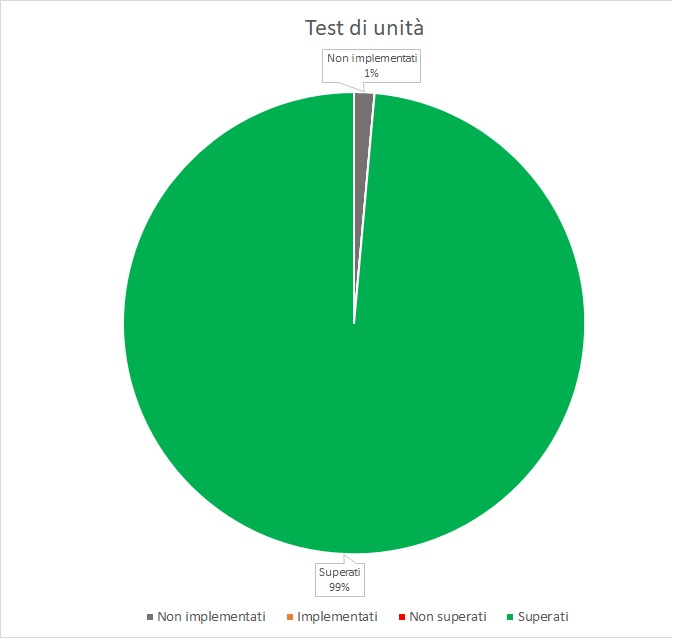
\includegraphics[scale=1]{Img/TU}
	\caption{Resoconto test di unità}\label{}
\end{figure}



\pagebreak